\section{Introduction}
This manual describes how to use the \RAS{} system together with the
\EMACS{} editor. It also describes how to obtain {\it persistence\/},
i.e. how to save results between sessions. Finally, it describes what
\RAS{} expressions look like, and what they mean. Basic familiarity
with \EMACS{} is assumed, cf. the {\sc Trine} manual.

\section{The Interpreter}
\label{theinterpreter}
The purpose of the \RAS{} interpreter is to evaluate expressions typed
by the user.   This chapter, describes the \RAS{} interpreter.

\subsection{Getting started}
\label{thewindowsystem}
To start \RAS{} from within \EMACS{}, use the \menu{Modes} menu. It has
two entries relating to \RAS{}:
\begin{itemize}
\bf
\item Rasmus
\item Rasmus...
\end{itemize}
The first entry will open up a new frame called {\tt RASMUS}, for the
communication with the \RAS{} interpreter. The second entry will start
by prompting for directories, before opening up the new frame, but is
otherwise identical to the first. The second entry will be further
explained in \chapterref{persistence}.

\samepage The \RAS{} frame contains a new menu, \menu{Rasmus} menu.
Its content looks something like \figureref{fig:rasmus-menu}.
%\begin{figure}[p]
\begin{figure}[H]
  \begin{center} \tt
    \begin{tabular}{|l|}
      \hline
      Evaluate\\
      Save last... \\
      Change name...\\
      Clean \\
      Modify\\
      Quit \\ 
      \hline
    \end{tabular}
  \end{center}
  \caption{The \menu{Rasmus} menu.}
  \label{fig:rasmus-menu}
\end{figure}
The explanation of \mopt{Evaluate} is described in the following,
while the explanation of \mopt{Save last...}~, \mopt{Change name...}
and \mopt{Clean} are deferred to \chapterref{persistence}. The
\mopt{Modify} entry will be described in a separate note.

\subsection{Getting along}
The \RAS{} frame consists of two separate parts (cf.
\figureref{initialinterpreter}). These parts are in the terminology of
\EMACS{} called \define{windows} (not to be confused with X-windows).
Each window has its own status-line. The top window is called the
\define{output} window, or the \define{passive} part. The bottom
window is called the \define{input} window or the \define{active}
part. Input to the interpreter is typed into the active window, and
the interpreter will respond in the passive window.
%\begin{figure}[h!p]
\begin{figure}[H]
%\centerline{\psfig{figure=rasfig-initial.ps}}
\centerline{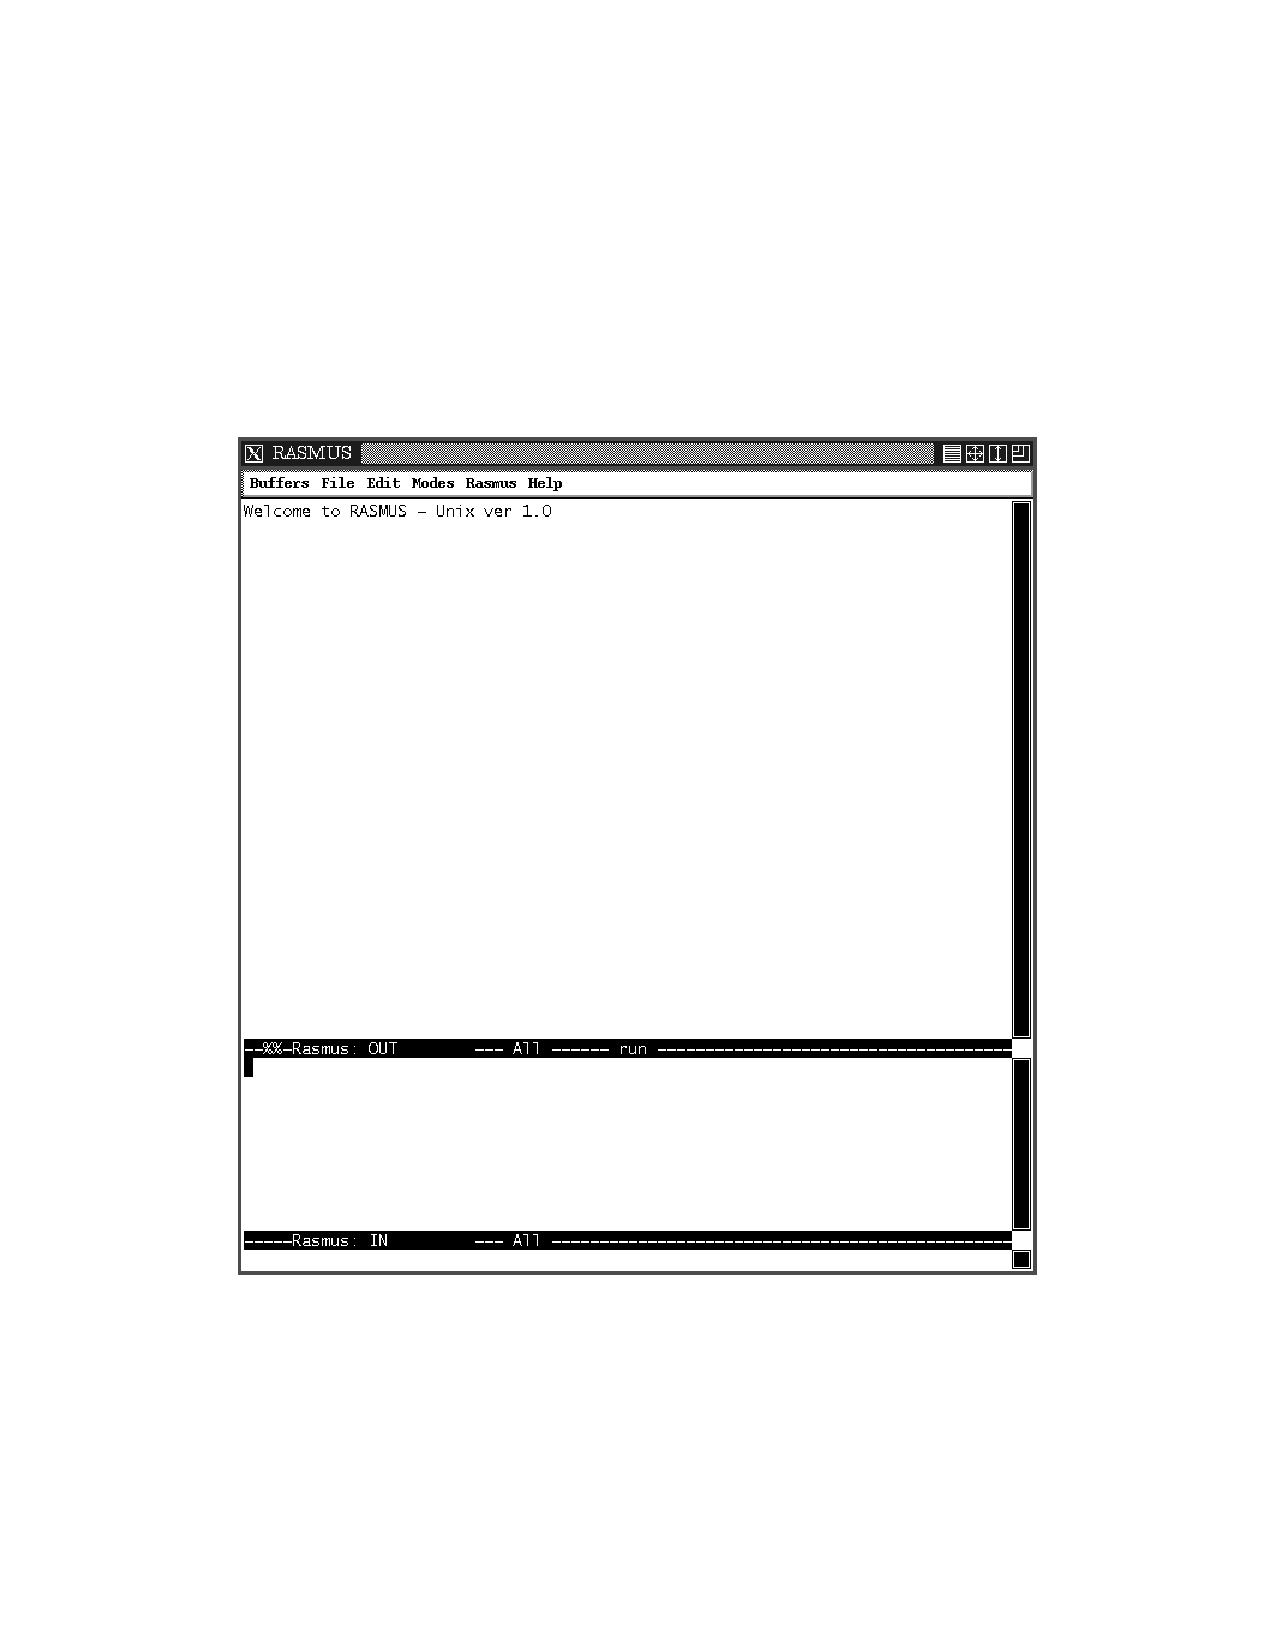
\includegraphics[]{rasfig-initial.pdf}}
\caption{Initial appearance of interpreter.}
\label{initialinterpreter}
\end{figure}

In fact, the active and passive windows are ordinary \EMACS{} buffers,
which operate in a special \RAS{} major mode. This means that anything
you can do with a buffer, you can also do with the \RAS{} windows,
including printing and saving.

In order to type in an expression for the interpreter to evaluate, the
input buffer must be made active. This is done either via the {\tt
  Buffers} menu, or by placing the cursor in the input window and
pressing the left mousebutton (you may also place the cursor in the
passive window, but the system will not allow you to alter the buffer
it displays).

Suppose you have typed in the following expression:
\begin{center}
\parbox{10em}{\tt
1+2+3+4+5+6+\\
7+8+9+10}
\end{center}
Your \RAS{} frame will now look as in \figureref{anexpininterpreter}.
\begin{figure}[p]
%\centerline{\psfig{figure=rasfig-firstexp.ps}}
\centerline{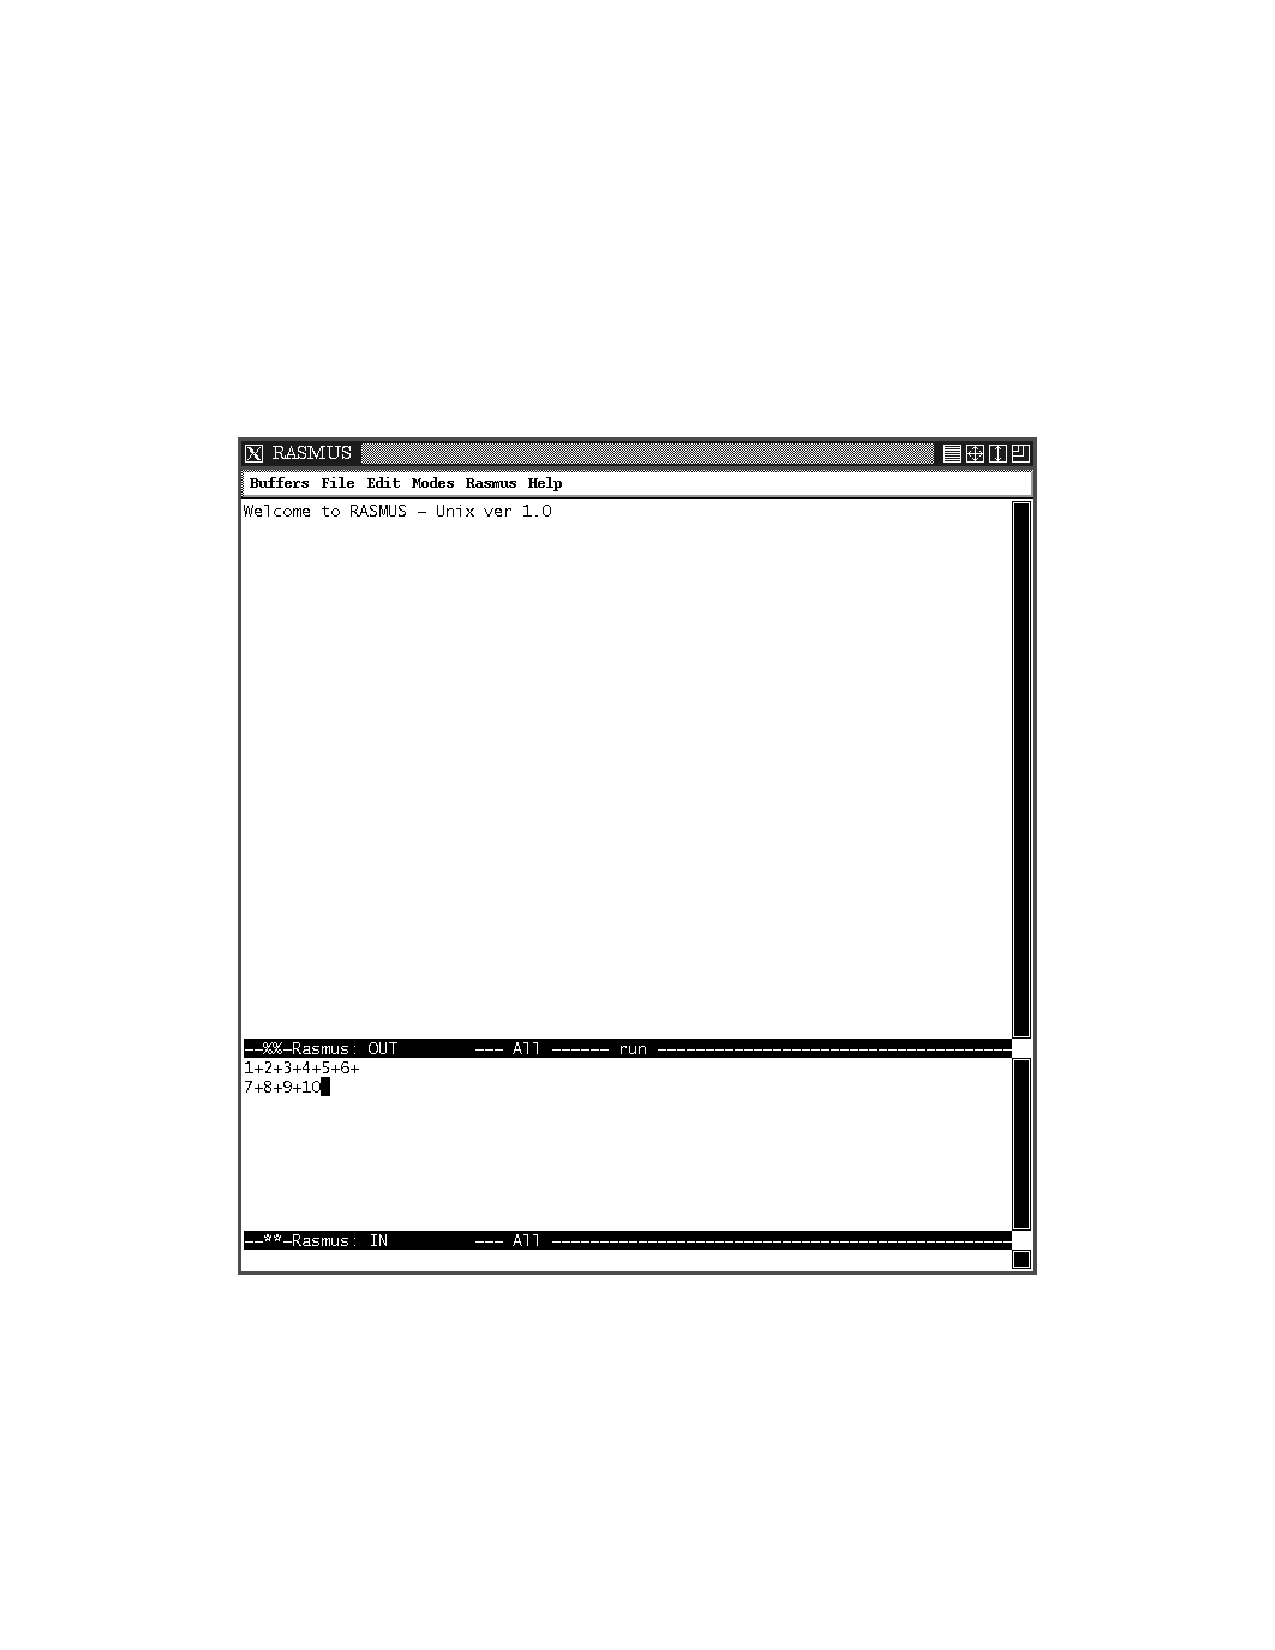
\includegraphics[]{rasfig-firstexp.pdf}}
\caption{Typing the first expression.}
\label{anexpininterpreter}
\end{figure}
In order to have the interpreter evaluate the expression, you must use
the \menu{Rasmus} menu. If you select \mopt{Evaluate}, your frame will
end up looking like \figureref{oneexpevaluated}.
\begin{figure}[p]
%\centerline{\psfig{figure=rasfig-firsteval.ps}}
\centerline{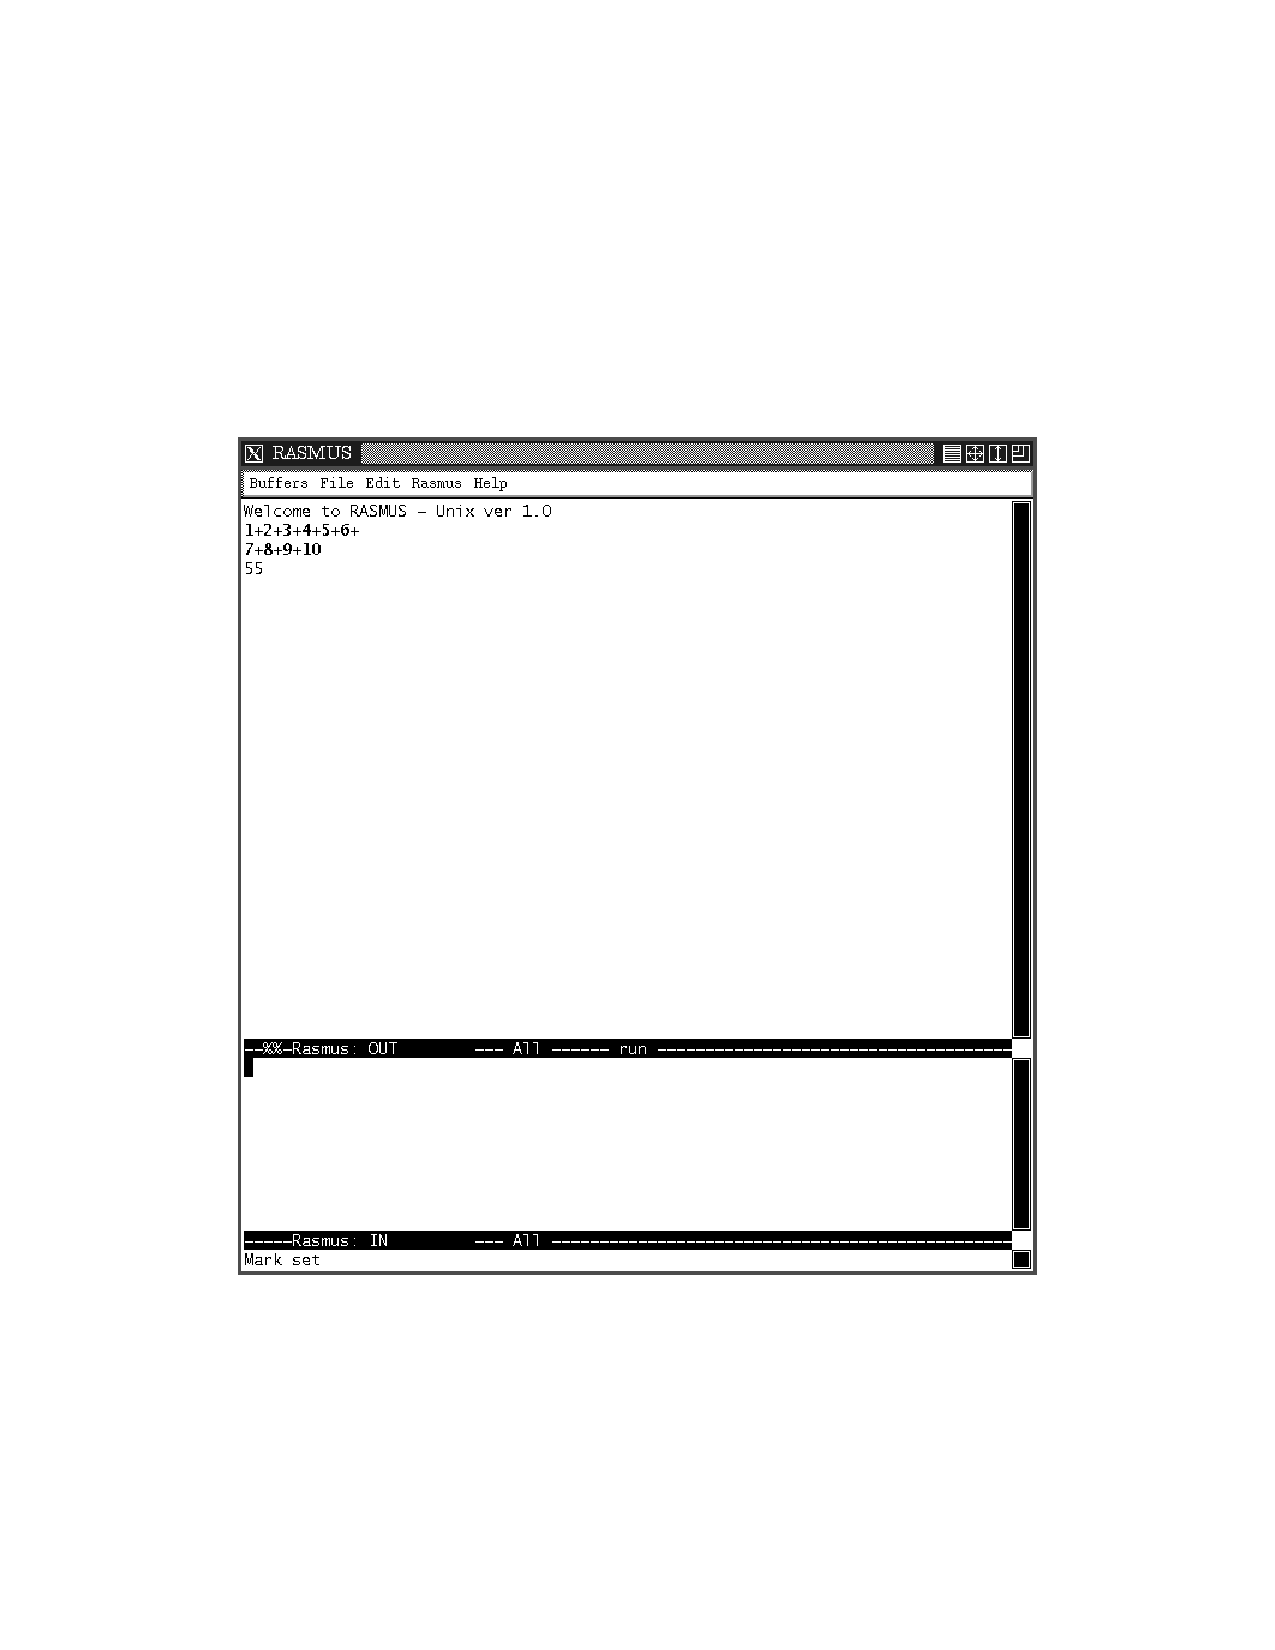
\includegraphics[]{rasfig-firsteval.pdf}}
\caption{After the evaluation.}
\label{oneexpevaluated}
\end{figure}
The expression has been copied from the active window into the passive,
using a different font, so that you may distinguish your input from
the output of the interpreter. The interpreter evaluates the
expression, and inserts the result into the output buffer. The active
window is then cleared.

If you have typed in an illegal expression, the active part is not
cleared, which means that you can edit the expression. What constitutes legal
expressions is further described in \chapterref{expressions}.

To get rid of the interpreter, you can use the \mopt{Quit} entry of the
\menu{Rasmus} menu. This will delete the {\tt RASMUS} frame and the
corresponding input and output buffers.
